\documentclass{standalone}
\usepackage{tikz}
\usepackage{ctex,siunitx}
\setCJKmainfont{Noto Serif CJK SC}
\usepackage{tkz-euclide}
\usepackage{amsmath}
\usetikzlibrary{patterns, calc,3d}
\usetikzlibrary {decorations.pathmorphing,decorations.pathreplacing,decorations.shapes}
\begin{document}
\small
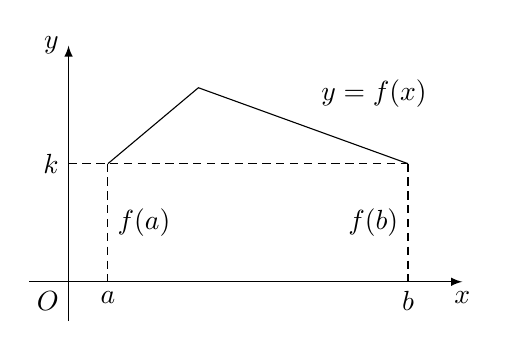
\begin{tikzpicture}[>=latex,scale=1.0]
  \draw[->](-0.5,0)--(5,0)node[below]{$x$};
  \draw[->](0,-0.5)--(0,3)node[left]{$y$};
  \draw(0.5,1.5)--++(40:1.5)--({0.5+2.2*sqrt(3)},1.5)node[midway,above right=0.15]{$y=f(x)$};
  \draw[densely dashed](0.5,1.5)--++(0,-1.5)node[below]{$a$}node[midway,right]{$f(a)$}({0.5+2.2*sqrt(3)},1.5)--++(0,-1.5)node[below]{$b$}node[midway,left]{$f(b)$}(0,1.5)node[left]{$k$}--({0.5+2.2*sqrt(3)},1.5);
  \node at (0,0)[below left]{$O$};
\end{tikzpicture}
\end{document}